\documentclass[11pt]{beamer}
\usetheme{Marburg}

\usepackage[utf8]{inputenc}
\usepackage[T1]{fontenc}
\usepackage[francais]{babel}
\usepackage{graphicx}

\author{Ashley Lesdalons \& Riyane Sid-Lakhdar}
\title{Autonomic Computing}
%\subtitle{}
%\logo{}
\institute{Adaptive Computing Systems}
\date{Tuesday 5, April}
%\subject{}
%\setbeamercovered{transparent}
%\setbeamertemplate{navigation symbols}{}

\addtobeamertemplate{navigation symbols}{}{%
    \usebeamerfont{footline}%
    \usebeamercolor[fg]{footline}%
    \hspace{1em}%
    \insertframenumber/\inserttotalframenumber
}

\AtBeginSection
{
  \begin{frame}<beamer>{Outline}
    \tableofcontents[currentsection,currentsubsection]
  \end{frame}
}

\begin{document}
	\maketitle

    
    \section{Definition of autonomic systems}
    \subsection{First approach of autonomic computing}
	\begin{frame}
		\frametitle{First approach of autonomic computing}
		\begin{center}
			\begin{itemize}
				\item "\textbf{\textit{Dealing with Autonomic Computing is reaching a totally new paradigm}}" [Paul Horn: IBM Senior Research VP, Harvard University, October 2001]
					\begin{itemize}
                    	\item From solving uni-case problems (smaller, faster, cheaper)
                        \item To building machines to solve future problems independently from the problem to solve
                    \end{itemize}

				\item Autonomic computing is not machine learning 

				\item Autonomic computing is dealing with the highly increasing need of hardware and software resources
			\end{itemize}
		\end{center}
	\end{frame}


    \subsection{Context and challenges}
	\begin{frame}
		\frametitle{Context and challenges}
		\begin{center}
            \begin{figure}[!htb]\centering
                \begin{minipage}{1.0\textwidth} \frame{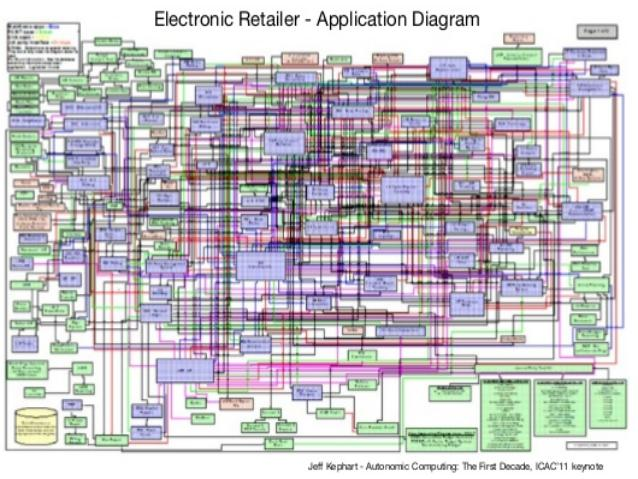
\includegraphics[width=\linewidth]{hardware-software-interaction-chaos.jpg}} \end{minipage}
                \caption{Interaction between hardware and software components}
                \label{hardware-software-interaction-chaos.png}
			\end{figure}
        \end{center}
    \end{frame}



    \subsection{Formal definition}
	\begin{frame}
		\frametitle{Formal definition}
		\begin{center}
				\item "\textbf{\textit{An autonomic computing system is an environment of distributed systems designed to host running software.   This software would seek for resource without considering the issues of providing them.}}"\newline
                [Autonomic Computing: The First Decade, IBM research corporation, 2001]
        

		\end{center}
    \end{frame}



\section{Key properties}
    \subsection{Properties on the hosted software}
	\begin{frame}
		\frametitle{Properties on the hosted software}
		\begin{center}
        \begin{itemize}
			\item The hosted software \textbf{\textit{ignores the existence or the characteristics of the host environment.}}"\newline
			\item Inspired from biological observations
		\end{itemize}
        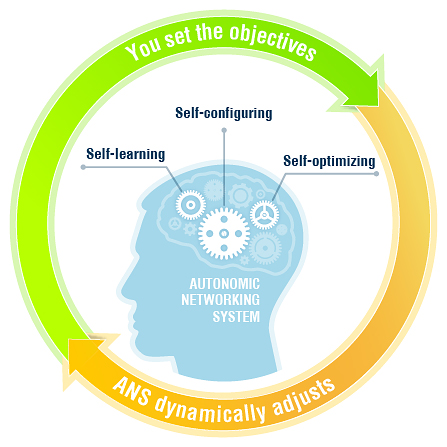
\includegraphics[scale=0.5]{ANS-BRAIN-2012.jpg}
		\end{center}
    \end{frame}

    \subsection{Properties of the autonomic system}
	\begin{frame}
		\frametitle{Properties of the autonomic system}
		\begin{center}
        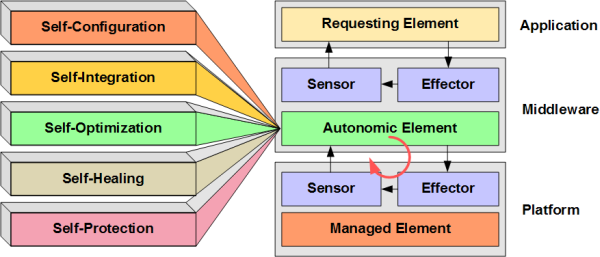
\includegraphics[scale=0.7]{propertiesAutonomicComputing.png}
		\end{center}
    \end{frame}

    \section{Architecture}
\begin{frame}
\frametitle{Autonomic manager}
\begin{itemize}
\item self-managing component of the system
\end{itemize}
\begin{center}
eferences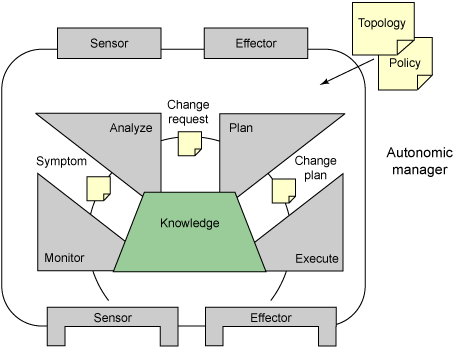
\includegraphics[scale=0.5]{autonomic-manager.png}
\end{center}
\end{frame}

    \subsection{Sensors}
\begin{frame}
\frametitle{Sensors}
\begin{definition}
An interface that exposes information about the state and state transitions of a managed resource.
\begin{example}
A user connects to www.example.com and tries to login. The sensor receives an error from the website application. (there are 2 users with the same credentials in the database).
\end{example}
\end{definition}
\end{frame}

	\subsection{Monitor}
\begin{frame}
\frametitle{Monitor}
The monitor provides the mechanisms that collect, aggregate, filter,
manage, and report details.
\newline
\begin{enumerate}
\item collect the details from the managed resources (sensors, effectors, logs...)
\item correlate them into symptoms that can be analyzed
\item store the distilled data in the knowledge base.
\end{enumerate}
\begin{example}
A user has two different entries with the same ID in the \textit{Users} table.
\end{example}
\end{frame}

    \subsection{Analyze function}
\begin{frame}
\frametitle{Analyze Function}
The analyze function provides the mechanisms to observe and analyze
situations to determine if some change needs to be made.\newline
\begin{itemize}
\item The analysis is influenced by stored knowledge data
\item If changes are required, the analyze function generates a change request and passes that change request to the plan function
\item two different levels of changes: necessary or desirable.
\end{itemize}
\end{frame}

\begin{frame}
\frametitle{Analyze Function}
\begin{example}
Policy = No duplicates in the \textit{Users} table.
A change is required: it is necessary to delete duplicate users
\end{example}
\end{frame}

    \subsection{Plan function}

\begin{frame}
\frametitle{Plan Function}
The plan function creates or selects a procedure to enact a desired alteration
in the managed resource.
\begin{itemize}
\item The plan is influenced by stored knowledge data
\item It creates a change plan and sends it to the execute function which will take care of applying the changes.
\end{itemize}
\begin{example}
The plan function identifies the duplicate users and keep only the first ones created. 
\end{example}
\end{frame}

    \subsection{Execute function}
\begin{frame}
\frametitle{Execute Function}
The execute function provides the mechanism to schedule and perform the
necessary changes to the system. \newline
\begin{example}
SQL queries are generated and then executed in the database.
\end{example}
\end{frame}
    
    \subsection{Knowledge}
\begin{frame}
\frametitle{Knowledge}
\begin{definition}
The knowledge is an implementation of a registry, dictionary,
database or other repository that provides access to knowledge according
to the interfaces prescribed by the architecture. It is shared between the different functions of the architecture.
\end{definition}
3 kind of knowledge:
\begin{itemize}
\item Solution Topology Knowledge
\item Policy Knowledge
\item Problem Determination Knowledge
\end{itemize}
\end{frame}

\begin{frame}
\frametitle{Data stored in the knowledge}
\begin{itemize}
\item topology information
\item historical logs
\item metrics
\item symptoms
\item policies
\item etc.
\end{itemize}
\begin{example}
Our knowledge contains:
\begin{itemize}
\item database containing the \textit{Users}
\item policy "no duplicate users"
\item change requests, change plans... 
\end{itemize}
\end{example}
\end{frame}
    
    \section{Recap and perspectives}
    \begin{frame}
        \frametitle{Overview}
        \begin{center}
        \begin{itemize}
			\item Autonomic computing has put the basis of modern distributes architecture (cluster, cloud computing, ...)
            \item IBM has leaded the autonomic computing researches by:
            \begin{itemize}
				\item Financing scholarships, and events all over the world
                \item Gathering all the scientific papers to identify the main trends and theoretical breakthrough
			\end{itemize}

            \item Analyzing the result of this researches has leaded to identify the main vision:
            \begin{itemize}
				\item Bio-inspired computing
                \item Recovery computing
			\end{itemize}
		\end{itemize}
		\end{center}
	\end{frame}

\begin{frame}
\frametitle{References}
\begin{itemize}
\item An architectural blueprint for autonomic computing, IBM, June 2005
\item A Practical Guide to the e to the IBM Autonomic Computing Toolkit Toolkit, Bart Jacob, Richard Lanyon-Hogg, Devaprasad K Nadgir, Amr F Yassin
\item Autonomic Computing, Hausi A. Müller, Liam O’Brien, Mark Klein, Bill Wood, April 2006
\item Autonomic Computing (Basics), http://www.slideshare.net/jaspreet93/autonomic-computing-basics-presentation
\item https://en.wikipedia.org/wiki/Autonomic\_computing
\end{itemize}
\end{frame}

\end{document}